Neste trabalho, foi implementado e avaliado um sistema fuzzy Takagi-Sugeno para a aproximação de uma função não linear, utilizando tanto consequentes constantes (ordem zero) quanto lineares (primeira ordem) e diferentes tipos de funções de pertinência (gaussiana, triangular e trapezoidal).

Os resultados demonstraram que o modelo de primeira ordem apresenta desempenho superior em relação ao de ordem zero, alcançando menores valores de RMSE para todas as funções de pertinência avaliadas. Destaca-se também que a otimização dos consequentes do modelo de ordem zero, por meio de gradiente descendente, proporcionou uma redução significativa do erro, tornando-o competitivo com o modelo de primeira ordem, especialmente quando utilizadas funções de pertinência triangulares.

Além disso, observou-se que a escolha adequada das funções de pertinência e o ajuste dos parâmetros do sistema são fundamentais para a qualidade da aproximação. O sistema Takagi-Sugeno mostrou-se eficiente e flexível, sendo capaz de aproximar funções não lineares com boa precisão mesmo com um número reduzido de regras.

Para ilustrar o impacto da otimização dos consequentes, a Figura~\ref{fig:erro_ordem_zero_otimizacao} apresenta os gráficos do erro antes e depois da otimização para cada tipo de função de pertinência no modelo de ordem zero.

\begin{figure}[!ht]
    \centering
    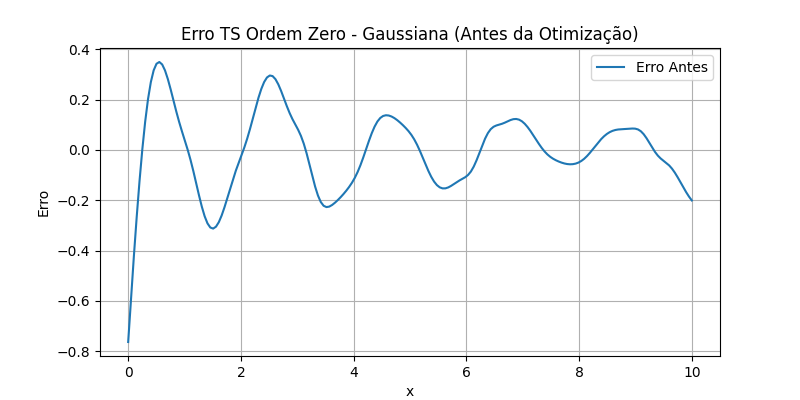
\includegraphics[width=0.32\textwidth]{../img/erro_ordem_zero_gaussiana_antes_takagi_sugeno2.png}
    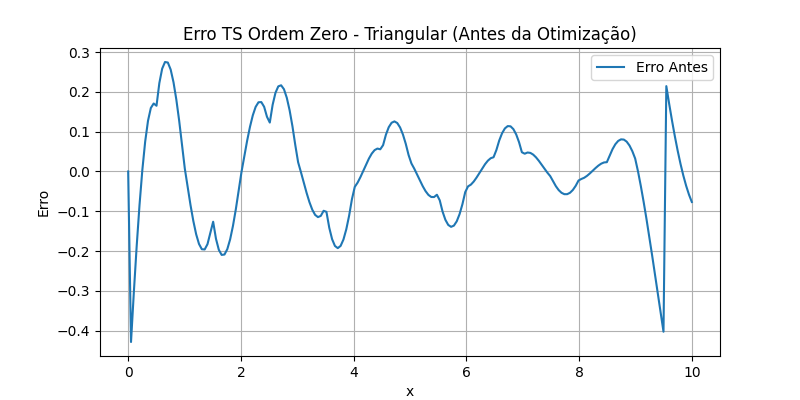
\includegraphics[width=0.32\textwidth]{../img/erro_ordem_zero_triangular_antes_takagi_sugeno2.png}
    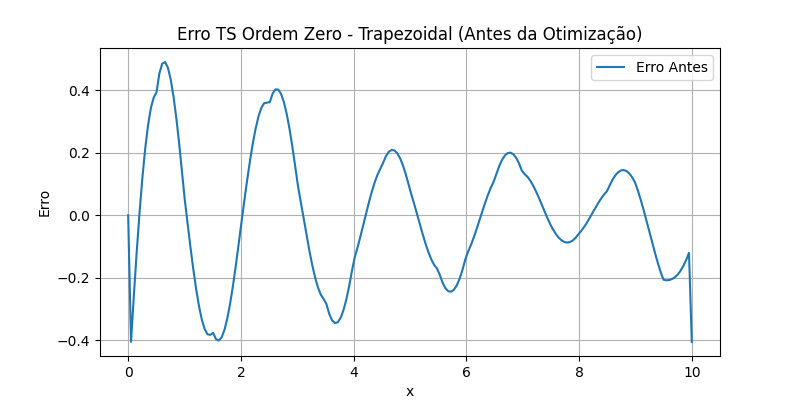
\includegraphics[width=0.32\textwidth]{../img/erro_ordem_zero_trapezoidal_antes_takagi_sugeno2.png}
    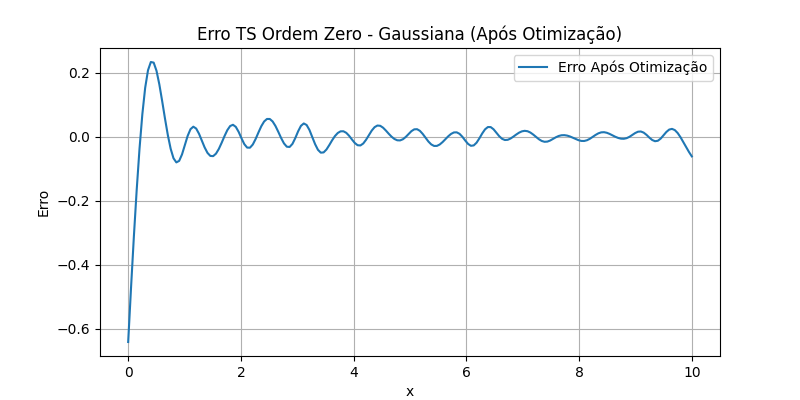
\includegraphics[width=0.32\textwidth]{../img/erro_ordem_zero_gaussiana_otimizada_takagi_sugeno2.png}
    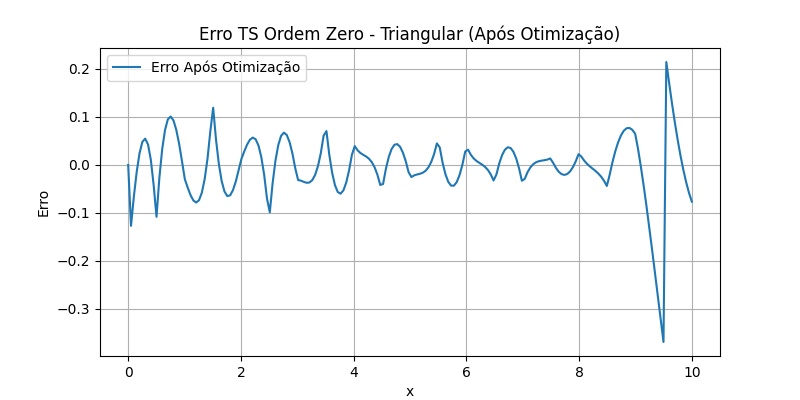
\includegraphics[width=0.32\textwidth]{../img/erro_ordem_zero_triangular_otimizada_takagi_sugeno2.png}
    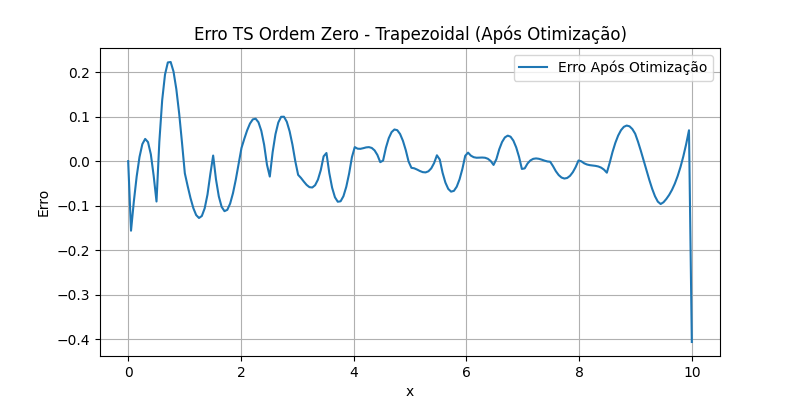
\includegraphics[width=0.32\textwidth]{../img/erro_ordem_zero_trapezoidal_otimizada_takagi_sugeno2.png}
    \caption{Erro do Takagi-Sugeno de ordem zero antes (linha superior) e após (linha inferior) a otimização dos consequentes para funções de pertinência gaussiana, triangular e trapezoidal.}
    \label{fig:erro_ordem_zero_otimizacao}
\end{figure}

Portanto, conclui-se que o modelo Takagi-Sugeno é uma ferramenta poderosa para problemas de aproximação de funções, e seu desempenho pode ser potencializado com técnicas de otimização e seleção criteriosa dos componentes fuzzy.